% Evaluation Chapter

\chapter[Evaluation]{Evaluation} % Main chapter title

\label{ChapterEvaluation} % For referencing the chapter elsewhere, use \ref{Chapter10} 

This chapter contains an evaluation of the swarm debugging system. The first portion of this evaluation is derived from the results of a number of `\textit{user evaluation sessions}' which are discussed in section \ref{UserEvaluationSessions}, and aim to determine the extent to which the system is useful in its intended context. The second portion is based on a comparison of the system with the aim and objectives of the project, as stated in section \ref{AimAndObjectives}.

%----------------------------------------------------------------------------------------

\section{User Evaluation Sessions} \label{UserEvaluationSessions}

Software testing can be used to verify that a system works as intended, however this does not guarantee that it is useful in practice. The purpose of the user evaluation sessions was therefore to determine whether or not the system satisfied its intended purpose. In order to do this, potential system users were asked to use the system to complete a number of tasks, and data was recorded regarding their experience. This data was obtained through direct observation of the participants interaction with the system, and through a follow up questionnaire designed to gauge their opinions on the system's various features and functionality. One of the stated objectives of the project was to build a system with a clear and intuitive user interface, hence a secondary purpose of the user evaluation sessions was to determine whether or not the user interface was intuitive to use and easy to navigate, without prior knowledge. It was therefore necessary to select participants who had no direct involvement in the development of the system, and were therefore not biased by an existing understanding of the user interface.

The user evaluation sessions followed an observed testing format. Participants were given full control of the system, which was initialised to a known state, and asked to complete a number of tasks, ranging from simple information and data location and retrieval to a full simulated debugging task. Data was collected by taking notes on how the participants interacted with the system, including any difficulties they had, and any comments they made whilst using it. The primary areas of interest for these notes were how easily the participant was able to navigate the user interface and obtain information, how often they asked for additional information, and what they asked for information regarding, as well as if (and how quickly) they were able to isolate and correct the deliberate behavioural fault during the debugging task, and what features of the system they made use of during their attempt.

\subsection{Participants}
Two groups of participants took part in the user evaluation sessions. The first was composed of `\textit{domain experts}'; researchers and other technical people with experience in the field of swarm robotics. This group were more likely to have an understanding of the needs of the system's target users, and therefore their input was considered more valuable. However because of the relatively niche nature of the field, the availability of participants in this category was limited. Hence only a small number could be found to participate in the sessions.

In order to remedy this lack of participants, the second group was introduced. This group was composed of undergraduate engineering students, who had a basic understanding of the core concepts of swarm robotics, but little or no practical experience. Where necessary an introduction to the core concepts was given before the session. This group did however possess general knowledge regarding software development, as this was necessary to complete the sessions effectively. The results obtained from this group were therefore mostly useful to evaluate elements of the system unrelated to swarm robotics, such as the usability of the user interface and the clarity of information display. This difference is reflected in the analysis of the results.

\subsection{Set Up}
Four robots were used during the sessions, each loaded with the same behaviours. Two simple behaviours were programmed for the robots prior to the start of the sessions. The first was a very simple data test behaviour which had the robot drive slowly in a circular path, whilst reporting data for all of the types defined in the system. This included a watchdog packet every ten control steps containing a unique name for each robot, a varying state which would change every fifty control steps between three possible values, active and background IR data, an arbitrary log message packet every hundred control steps and a custom data packet every ten control steps, containing the current total number of control steps as its data. 

The second behaviour was a simple dispersion behaviour, which would cause the robot to turn and drive away from any nearby object. This was achieved by monitoring the values of the robots IR sensors, calculating a vector of highest IR reflection intensity based on these values, and negating it to acquire a heading vector in the opposite direction. Sensor values were only included in the reflection intensity vector calculation if they surpassed a specific threshold, in an attempt to eliminate the effects of random noise. Whilst executing this behaviour the robot was also reporting debugging information to the application. This included watchdog packets, active and passive IR data, and the control step as custom data all as before, as well as the state of the robot which would vary between \textit{IDLE} and \textit{MOVING}. In order to simulate a bug in the robot's behaviour code, the IR value threshold in this second behaviour was deliberately set too low, causing the robots to move randomly when no objects were nearby, as a result of the fluctuations in the IR readings due to noise. A further consequence of this was that the robot would rarely, if ever, enter the \textit{IDLE} state. Participants were then asked to attempt to locate the cause of this bug using the debugging system.

Prior to the start of each session the robots were returned to their initial state, with the two behaviours loaded and the first behaviour running. The application was not set up in any way, and was run fresh for each session. It was important that this starting set up be the same for each participant, in order for the results to be comparable.

\subsection{Session Sequence}
The following sequence of steps was then carried out for each session. Participants were deliberately not told precisely where to find specific information, or exactly how to complete each task, in order to observe the extent to which the user interface was intuitive. Participants were asked to say if they could not determine how to complete one of the tasks, at which point further guidance was given. Relevant observational notes were taken at each step.

\begin{enumerate}
 \item Introduce the application to the participant, and have them run the executable.
 \item Explain the purpose of the application, and the purpose of this evaluation session.
 \item Indicate the key features within the application. Specifically identify the visualiser and explain its purpose, as well as the robot list panel and the data panel.
 \item Ask the participant to start the application listening for data packets on the network. Mention that this functionality can be found on the network tab only if necessary.
 \item The simple circular motion controller code should be running on the robots already. If it is not, run it now.
 \item Ask the participant to obtain the following pieces of information:
 \begin{enumerate}
  \item The current state of robot 1
  \item The recent state changes of robot 2
  \item The current IR sensor values of robot 3
  \item The current value of the `ControlStep' custom data point for robot 4
  \item The set of known states for robot 1
  \item The numerical angle describing the orientation of robot 2
 \end{enumerate}
 \item Ask the participant to use the visualiser settings tab to achieve the following:
 \begin{enumerate}
  \item Hide the name and state visualisation for all robots
  \item Display the recent path for all robots
  \item Display the IR sensor data for the selected robot in heat mode
  \item Hide the position and orientation visualisation for all robots
  \item Display the custom data point `ControlStep' for the selected robot.
 \end{enumerate}
 \item Ask the participant to use the camera settings tab to add a mapping from ARuCo tag ID 2 to robot ID 10. Explain further if necessary.
 \item Ask the participant to use the logging tab to achieve the following:
 \begin{enumerate}
  \item Set the logging directory to a specific folder
  \item Start logging for a short period of time and then stop it.
 \end{enumerate}
 \item Stop the circular motion behaviour on the robots and switch to the dispersion behaviour.
 \item Make the dispersion behaviour source code available to the user.
 \item Explain the desired behaviour to the participant, and the current erroneous behaviour.
 \item Ask the participant to attempt to locate the cause of the issue using the data made available by the debugging system. Provide hints and advice only if necessary.
\end{enumerate}

\subsection{Observations}
The following is a summary of the observations and comments made during the evaluation sessions. Special note was taken of any observation or comment made by more than one participant. Steps in the session for which no comments are noted can be assumed to have been completed without issue by all participants.

All participants were able to quickly find the network tab and enable packet listening, at which point the system began receiving data from the robots. All participants were also able to easily locate all of the requested information. The only exception to this was the current state of robot 1, which three of the participants commented was not clearly displayed on the state tab. The state tab displays other state related information, but does not clearly display the current state (it can be inferred from the state transition list), which was an oversight in the user interface design. All participants were able to subsequently locate the current state on the overview tab.

All participants were able to locate the visualiser settings tab and determine how to enable and disable visualisations. Three of the participants were initially confused by the fact that the visualiser settings were unrelated to the selected robot, instead applying globally. Five participants also commented that the process of double clicking an item within the visualiser configuration list, to access the more specific settings, was unintuitive. Several commented that this was not a user interface behaviour they had seen before, and therefore was not immediately obvious. Suggested alternatives were to use drop-down menus, a right click menu, or a `tree' style expandable list, to access detailed settings for each visualisation. One participant also commented that the detailed settings for the IR data visualisation were not clearly described, especially regarding the two possible modes; proximity mode and heat mode. They commented that these would be better presented as a drop-down selector.

During the simulated debugging task all participants made use of the visualiser settings to configure the way that data was displayed, and used the visualiser display when attempting to determine the cause of the issue. Three participants adjusted the visualiser settings more than once. Five participants used the state tab to identify that the robots were incorrectly remaining in the \textit{HEADING} state, and not moving to the \textit{IDLE} state as the code suggested they should. All six participants used the IR data tab to check the values being reported by the robots' IR sensors, and all six were able to identify that the cause of the bug was the low threshold value. As expected the members of the domain expert participant group were quicker to locate the simulated bug than those in the non-expert group. One participant from the non-expert group explicitly noted that familiarity with the robots and their basic capabilities would have made the task significantly easier.

All three members of the domain expert group commented on their belief that the system would be useful, based on their prior experience with swarm robotics. One participant specifically mentioned the system's applicability to their current work, and noted a number of scenarios where the custom data reporting functionality would be useful, including reporting `pheromone' levels in a swarm path-finding behaviour. Another member of the expert group commented that they liked the idea of re-using the system with a different robot platform, and noted that the use of the \textit{ArUco} tracking tags would improve the ease of the porting process. The three members of the non-expert group each identified the IR and state data reporting as useful in completing the simulated debugging task.

\subsection{Questionnaire}
Following the practical session, participants were asked to complete a questionnaire regarding their experience, and their opinions of the system and its features. The questionnaire included the following questions:

\noindent\textbf{Question 1: How would you rate your overall impression of the user interface?}\\(Scale of 1 to 5, `poor' to `excellent')

\begin{center}
\begin{tabular}{ l c c c c c c }
 Group & 1 & 2 & 3 & 4 & 5 & Average Score \\ 
 \hline
 Domain Experts & 0 & 0 & 0 & 1 & 2 & 4.7 \\
 Others 		& 0 & 0 & 0 & 2 & 1 & 4.3 \\
\end{tabular}
\end{center}

\noindent\textbf{Question 2: How intuitive was the robot selection mechanism?}\\(Scale of 1 to 5, `not intuitive at all' to `highly intuitive')

\begin{center}
\begin{tabular}{ l c c c c c c }
 Group & 1 & 2 & 3 & 4 & 5 & Average Score \\ 
 \hline
 Domain Experts & 0 & 0 & 0 & 0 & 3 & 5 \\
 Others 		& 0 & 0 & 0 & 1 & 2 & 4.7 \\
\end{tabular}
\end{center}

\noindent\textbf{Question 3: How easy was it to locate the requested information?}\\(Scale of 1 to 5, `very hard' to `very easy')

\begin{center}
\begin{tabular}{ l c c c c c c }
 Group & 1 & 2 & 3 & 4 & 5 & Average \\ 
 \hline
 Domain Experts & 0 & 0 & 0 & 0 & 3 & 5 \\
 Others 		& 0 & 0 & 0 & 1 & 2 & 4.7 \\
\end{tabular}
\end{center}

\noindent\textbf{Question 4: How would you rate the organisation of information in the lower data panel?}\\(Scale of 1 to 5, `poorly organised' to `well organised')

\begin{center}
\begin{tabular}{ l c c c c c c }
 Group & 1 & 2 & 3 & 4 & 5 & Average \\ 
 \hline
 Domain Experts & 0 & 0 & 0 & 1 & 2 & 4.7 \\
 Others 		& 0 & 0 & 0 & 1 & 2 & 4.7 \\
\end{tabular}
\end{center}

\clearpage
\noindent\textbf{Question 5: For each of the following data types, how would you rate their presentation within the visualiser, in terms of information clarity?}

\begin{figure}[h]
	\centering
	\makebox[\textwidth][c]{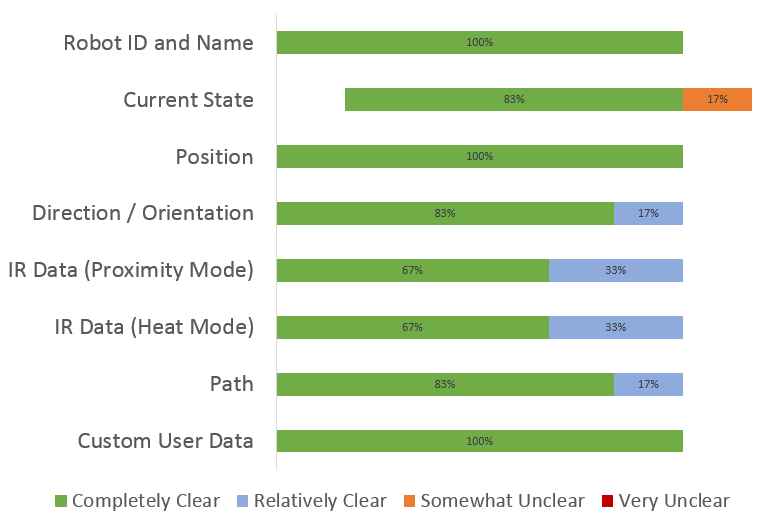
\includegraphics[scale=0.6]{VisualisationLikert.png}}
	\decoRule
	\caption[Evaluation Questionnaire Question 5 Results]{The results of Question 5.}
	\label{fig:VisualisationLikert}
\end{figure}

\noindent\textbf{Question 6: How easy was it to adjust the visualiser settings as requested?}\\(Scale of 1 to 5, `very easy' to `very difficult')

\begin{center}
\begin{tabular}{ l c c c c c c }
 Group & 1 & 2 & 3 & 4 & 5 & Average \\ 
 \hline
 Domain Experts & 0 & 0 & 0 & 1 & 2 & 4.7 \\
 Others 		& 0 & 0 & 0 & 1 & 2 & 4.7 \\
\end{tabular}
\end{center}

\noindent\textbf{Question 7: How beneficial do you believe the visualiser component to be to the overall application functionality?}\\(Scale of 1 to 5, `not beneficial at all' to `essential')

\begin{center}
\begin{tabular}{ l c c c c c c }
 Group & 1 & 2 & 3 & 4 & 5 & Average \\ 
 \hline
 Domain Experts & 0 & 0 & 0 & 0 & 3 & 5 \\
 Others 		& 0 & 0 & 0 & 1 & 2 & 4.7 \\
\end{tabular}
\end{center}

\noindent\textbf{Question 8: How easy / clear was it to use the network tab to begin listening for robot data packets?}\\(Scale of 1 to 5, `very difficult / unclear' to `very easy / clear')

\begin{center}
\begin{tabular}{ l c c c c c c }
 Group & 1 & 2 & 3 & 4 & 5 & Average \\ 
 \hline
 Domain Experts & 0 & 0 & 0 & 0 & 3 & 5 \\
 Others 		& 0 & 0 & 0 & 0 & 3 & 5 \\
\end{tabular}
\end{center}

\noindent\textbf{Question 9: How easy / clear was it to use the logging tab to record received data to a log file?}\\(Scale of 1 to 5, `very difficult / unclear' to `very easy / clear')

\begin{center}
\begin{tabular}{ l c c c c c c }
 Group & 1 & 2 & 3 & 4 & 5 & Average \\ 
 \hline
 Domain Experts & 0 & 0 & 0 & 1 & 2 & 4.7 \\
 Others 		& 0 & 0 & 0 & 0 & 3 & 5 \\
\end{tabular}
\end{center}

\noindent\textbf{Question 10: How would you rate your overall impression of the system's usefulness as a debugging tool?}\\(Scale of 1 to 5, `not useful at all' to `extremely useful')

\begin{center}
\begin{tabular}{ l c c c c c c }
 Group & 1 & 2 & 3 & 4 & 5 & Average \\ 
 \hline
 Domain Experts & 0 & 0 & 0 & 0 & 3 & 5 \\
 Others 		& 0 & 0 & 0 & 1 & 2 & 4.7 \\
\end{tabular}
\end{center}

\noindent\textbf{Question 11: Please feel free to add any additional comments regarding any aspect of the system.}
\begin{itemize}
 \item ``\textit{Drop down menu to choose single robot/all robots would be a nice addition. More visual "heat mode" display against dark background would also be useful.}''
 \item ``\textit{This seems like an extremely useful addition to the system. I can see how debugging without this application would be much harder and take much longer.}''
 \item ``\textit{Exceptionally useful system with intuitive and easy to use interface; shows a high level of polish and thought in UI design. Naturally some areas could have subtle improvements but nothing major!}''
 \item ``\textit{Really intuitive to use and I can already think of multiple use cases where this will be beneficial for robot lab researchers. Updated quickly and software seemed to run seamlessly. Ability to monitor custom data will be incredibly useful too. Loved how data was displayed in bar charts in the bottom panel and the heat mode display of the IR sensors. Excellent way to display information visually for quick diagnosis of problems. Literally only thing I found that wasn't immediately intuitive was the additional settings on the Visualizer Settings.}''
\end{itemize}

%----------------------------------------------------------------------------------------

\subsection{Analysis}
A general appraisal of the observations and comments made during the evaluation sessions, and the responses to the subsequent questionnaire, indicates an overall positive response to system. Participants were able to easily navigate and use the majority of the UI, without detailed direction, indicating that the user interface is intuitive and clear. The following remedies for minor issues with the user interface should be applied:

\begin{itemize}
 \item The interface for accessing specific visualisation settings should to conform to a more commonly seen interface pattern. An expandable list would work well, with main list items for each of the visualisations, and sub-items attached to each for specific settings.
 \item The current state should be displayed clearly on the state tab, possibly by highlighting the current state within the known state list.
 \item The IR data visualisation modes selection should be changed to use a drop-down menu selector.
\end{itemize}

The participants use of the system during the simulated debugging task, including examining state changes and IR data, and utilising the visualiser settings, coupled with their comments, suggests that the system is useful in practice. This aligns with the high scores for usefulness that the system received in responses to question ten of the questionnaire. Comments from the domain expert group of participants regarding the potential use of the system in their swarm robotics work also reflect well on the system, suggesting that these participants believe they can benefit from its use. The specific use of the visualiser by the participants, and the high scores in response to question seven, indicate that the system benefits from the inclusion of the visualiser, and is more useful than a data reporting system without a visual component.

Overall the results of the user evaluation sessions were positive, suggesting that the system meets the two key objectives being examined in these sessions; being useful in a practical debugging context, and displaying information through an intuitive interface. However the limited sizes of the participant groups and the simulated nature of the debugging task restrict the extent to which conclusions can be drawn from this study. Further usage of the system by a larger number of researchers, and in real debugging scenarios, would be necessary to get a more reliable idea of its value as a swarm debugging tool.

%----------------------------------------------------------------------------------------

\section{Comparison with Project Aim and Objectives}

In order to evaluate the success of the project overall each of the objectives stated in \ref{AimAndObjectives} can be compared against the project outcome.

\noindent \textbf{Utilise existing fiducial marker based tracking technology to track the position of individual robots within a swarm over time.}

The system utilises the ArUco tag detection system and camera set up described in section \ref{TrackingHardware} to track the positions and orientations of the robots in real time. This is enabled by the \textit{CameraController} and \textit{MachineVision} classes of the application, discussed in section \ref{VideoFeedAndTrackingSystem}. The ability of the system to accurately track the robots' positions was verified numerous times during the user interface testing process, including during the testing of the visualiser component's position and direction overlays, described in section \ref{ManualUserInterfaceTesting}, and in test C3 of the verification testing, described in section \ref{ValidationTesting}. This objective was therefore met successfully.

\noindent \textbf{Develop code to allow multiple robots to communicate information regarding their internal state, sensor readings and decision making to a central application wirelessly via a network.}

The system utilises a WiFi network to enable data transfer from the robots to the application. The code controlling the networking functionality of the application, enabling the receiving of data, is discussed in section \ref{Networking}. The code controlling the networking functionality on the robot side, enabling the sending of a robot's data, is discussed in section \ref{RobotSide}. Test C2 and C7 of the verification testing process, described in section \ref{ValidationTesting}, verify that the networking functionalities of both sides operate correctly, and that data is transferred correctly. This objective was met successfully.

\noindent \textbf{Develop a data model that allows the central application to store information received from the robots, and update it as new information arrives.}

The design for the application data model is presented in section \ref{DataModelDesign}. This design was then used during the implementation of the data model, which is discussed in section \ref{DataModel}. The data model component was tested using a unit-testing style methodology, which is discussed in section \ref{BackEndUnitTesting}, and the correct operation of the component was verified. The results of test case C7 and by extension test cases C5 and C6 in the validation testing process, described in section \ref{ValidationTesting}, verify that the data model functions correctly when used in conjunction with the other application components. This objective was therefore met successfully.

\noindent \textbf{Develop code to ascertain higher level data related to the robots, such as recent movement history or state transition history, and add this data to the model.}

The application data model includes support for storing robots' recent movement and state transition histories, as discussed in section \ref{DataModel}. The \textit{Position History Test} and the \textit{State History Test} in the data model unit testing campaign, described in section \ref{BackEndUnitTesting}, verify the correct storage of these data points in the data model, hence this objective was met successfully.

\noindent \textbf{Design and implement a user interface which is easy and intuitive to use, and presents data from the data model to the user in a human readable manner.}

The design of the user interface is discussed in section \ref{UserInterfaceDesign}, and its implementation is discussed in \ref{UserInterfaceImplementation}. During both stages usability, readability, and the clear presentation of data were primary concerns. The manual user interface testing process, described in section \ref{ManualUserInterfaceTesting}, verified that the interface itself and all data displayed was readable, clear and sensibly arranged. The user evaluation sessions, described in section \ref{UserEvaluationSessions} went on to suggest that, among a small sample of both expert and non-expert users, the interface was intuitive and easy to use. Feedback regarding the interface was overwhelmingly positive, in spite of some minor issues being raised regarding some settings-related interface controls. Overall the testing and user evaluation results indicate that this objective was met successfully.

\noindent \textbf{Develop a visual display component for the central application, which presents the user with a live video feed of the robot swarm, augmented with relevant and spatially situated information relating to the robots, by fusing data obtained from the robots with data obtained from the tracking system.}

The visualiser component satisfies the requirement for an augmented-reality style, graphical data visualisation component. The software design of the visualiser is discussed in section \ref{VisualiserDesign}, whilst the design of the appearance of the visualiser and the individual data visualisations is discussed in section \ref{DataVisualisationDesigns}. The implementation of the visualiser component is discussed in \ref{VisualiserImplementation}. The visualiser portion of the manual user interface testing process, discussed in section \ref{ManualUserInterfaceTesting} verified that the visualiser could correctly combine tracking data, robot data and the video feed to present spatially situated graphical and textual data representations, satisfying this objective. Furthermore, the results and feedback from the user evaluation sessions indicated that users responded positively to the graphical representations of data, and believed the inclusion of the visualiser component significantly benefited the application.

\noindent \textbf{Develop the user interface in such a way as to allow the user to filter out information that is not currently relevant, and to contrast and compare information related to specific robots.}

Information filtering within the visualiser component is achieved through the visualiser settings tab, discussed in section \ref{VisualiserImplementation}. For data outside the visualiser, filtering is achieved simply through selecting a target robot, and a specific data tab, using the interface described in section \ref{UserInterfaceImplementation}. The manual user interface testing process, described in section \ref{ManualUserInterfaceTesting}, verified that data filtering within the application worked correctly. During the user evaluation sessions, described in section \ref{UserEvaluationSessions}, participants were able to correctly filter visualiser data displays when asked, and used this feature a number of times during the simulated debugging task, suggesting that the portion of this objective relating to information filtering was met successfully. The latter portion, relating to robot data comparison was not met, as this objective was dropped following the initial survey which indicated a low desire for comparison features among potential system users.

\noindent \textbf{Design and implement the system in a modular way so as to allow for relatively simple integration with other swarm robotic platforms and tracking systems in future extensions.}

Modularity is achieved within the system in a number of ways. Firstly the use of a standardised data transfer format as discussed in section \ref{DataTransferFormat}, which is not specific to a single robot platform, ensures that data from any source can be interpreted correctly by the application. This was verified in test S2 of the verification testing process, discussed in section \ref{ValidationTesting}. The choice of WiFi as the networking technology, discussed in section \ref{Networking}, also helps to ensure portability due to WiFi's widespread use. The \textit{CameraController} and \textit{MachineVision} application components were also implemented in a modular fashion, as discussed in section \ref{VideoFeedAndTrackingSystem}, allowing for other camera drivers to be used with minor modification to the application source code. Furthermore tracking data is incorporated into the standard data transfer format, and can therefore be received via the network. Hence a developer using a different could tracking system could implement code to send their tracking data to application via the network, bypassing the \textit{CameraController} or \textit{MachineVision} components, and allowing completely different camera and tracking hardware to be used. Standard testing procedures could not be used to verify the portability or extensibility of the system, however during the user evaluation sessions one participant from the domain expert group specifically remarked on the ease with which the system could be transferred to another robot platform, due to the use of the hardware-less ArUco tags for tracking, and the non-robot-specific implementation of the robot side API for data reporting. Collectively these factors indicate that this objective was met successfully.

%----------------------------------------------------------------------------------------

\section{System Limitations}

In spite of the projects success in achieving the aims and producing a working system, a number of limitations inherent to the systems nature have been identified and are summarised here.

\begin{description}
 \item [Effect on robot behaviour.] In order to receive data from the robots, the system requires that   additions are made to the robot's controller code to report this data. Any time code is added to the robot's controller it has the potential to effect the behaviour in unforeseen ways, even if the added code has no direct effect on the code controlling decision making. This is because time is required to execute the data reporting code, and this can have a knock on effect on the execution of the rest of the code. This is most dangerous when deploying a swarm system, as the developer may choose to remove all of the data reporting code prior to producing the `release' version of the system, as this code is debugging focused, and not needed in a final version once correct operation has been established. If there is a significant amount of data reporting code, removing it all could have a non-negligible effect on the robots behaviour, leading to potential unpredictability. In order to mitigate this problem as much as possible the robot side code has been implemented to require as little time as possible to transmit data packets.
 
\item [WiFi network requirement.] The system requires that all robots be connected to one WiFi network in order to operate correctly. This means the current system is limited to robots which can support WiFi, and requires that the network infrastructure be in place. Considering the system's intention as a debugging tool, and therefore its likely use within laboratories, WiFi network infrastructure is not an unreasonable requirement. However not all robot platforms support WiFi, hence this system in its current state is limited to robot platforms that do. Section \ref{HardwareExpansion} discusses extending the system in future to support a further wireless protocol such as Bluetooth.

\item [Fixed Camera Viewpoint.] The video based portion of the system has been implemented to function with the video captured from a fixed viewpoint, with an overhead, birds-eye view of the robots. The system cannot correctly augment the video if it is captured from any other angle, even though the tag detection algorithm can cope with a range of angles. The system is therefore limited to consider and augment the space in only be two dimensions, and cannot display height-related data in any way. Many consider a three-dimensional reference frame to be a requirement of a true augmented-reality system \cite{Azuma:1997}, \cite{Billinghurst:2014}, and this system would have to be modified to support a non-specific viewpoint in order to work with modern augmented reality hardware.
\end{description}

%----------------------------------------------------------------------------------------
